\documentclass[12pt, a4paper, oneside]{ctexart}
\usepackage{amsmath, amsthm, amssymb, bm, graphicx, hyperref, mathrsfs}

\title{\textbf{HW3}}
\author{方科晨}
\date{\today}
\linespread{1.5}
\newcounter{problemname}
\newenvironment{problem}{\stepcounter{problemname}\par\noindent\textbf{Problem\arabic{problemname}. }}{\\\par}
\newenvironment{solution}{\par\noindent\textbf{Solution. }}{\\\par}
\newenvironment{note}{\par\noindent\textbf{题目\arabic{problemname}的注记. }}{\\\par}

\begin{document}

\maketitle

\begin{problem}
    
    \textbf{(a)} 要最小化 $\Vert Ax-b\Vert_\infty=\max_i (Ax-b)_i$ ,则有线性规划如下:
    $$\begin{array}{ll}
        \textrm{minimize} & c\\
        \textrm{subject to} &Ax-b\leq c\cdot e
    \end{array}$$ 其中 $e$ 为全 $1$ 向量。由于要最小化 $c$ ,则限制条件中必有一维取等号,此时 $c=\Vert Ax-b\Vert_\infty$ ,故两者等价。

    \textbf{(b)} 要最小化 $\Vert Ax-b\Vert_1=\sum_i|Ax-b|_i$ 。我们有如下的线性规划:
    $$\begin{array}{ll}
        \textrm{minimize} & \sum_i (y_i+z_i)\\
        \textrm{subject to} & Ax-b=y-z\\
        & y\geq 0\\
        & z\geq 0
    \end{array}$$
    不难发现这对于每一维来说 $y_i,z_i$ 都是独立的。对于每一维 $i$ 来说,有 $(Ax-b)_i=y_i-z_i$ ,假设 $y_i>0,z_i>0$ ,则存在一个 $0< a\leq \min(y_i,z_i)$ 使得 $y_i-a\geq 0,z_i-a\geq 0,(Ax-b)_i=(y_i-a)-(z_i-a)$ 满足限制条件,而且同时有 $(y_i-a)+(z_i-a)<y_i+z_i$ ,这样肯定不是最优解。故对于每一维 $i$ ,都有 $y_i=0,z_i=0$ 中的一个成立,则只有两种情况 $y_i=0,z_i=-(Ax-b)_i=|Ax-b|_i\geq 0$ 或者 $y_i=(Ax-b)_i=|Ax-b|_i\geq 0,z_i=0$ ,则 $y_i+z_i=|Ax-b|_i$ 。那么 $\sum_i(y_i+z_i)$ 正是我们要求的 $\Vert Ax-b\Vert_1$ ,故两问题等价。

    \textbf{(c)} 我们有以下线性规划问题:
    $$\begin{array}{ll}
        \textrm{minimize} & \sum_i(y_i+z_i)\\
        \textrm{subject to} & Ax=b\\
        & x=y-z\\
        & y\geq 0\\
        & z\geq 0
    \end{array}$$ 等价性的证明同理于 \textbf{(b)} 。
\end{problem}

\begin{problem}

    \textbf{(a)} 令 $|x|=x_1-x_2,|y|=x_3-x_4$ ,转化后有如下标准型:
    $$\begin{array}{ll}
        \textrm{minimize} & c^Tx\\
        \textrm{subject to} & Ax=b\\
        & x\geq 0
    \end{array}$$
    其中 $x=\begin{pmatrix}x_1\\ \vdots\\x_6\end{pmatrix},c=(1,1,1,1,0,0),A=\begin{pmatrix}
        1 & -1 & 1 & -1 & -1 & 0\\
        1 & -1 & 0 & 0 & 0 & 1
    \end{pmatrix},\\b=\begin{pmatrix}
        2\\
        3
    \end{pmatrix}$

    \textbf{(b)} 令 $x=x_1,y=x_2-x_3,z=x_4$ ,转化后有如下标准型:
    $$\begin{array}{ll}
        \textrm{minimize} & c^Tx\\
        \textrm{subject to} & Ax=b\\
        & x\geq 0
    \end{array}$$
    其中 $x=\begin{pmatrix}
        x_1\\ \vdots \\ x_8
    \end{pmatrix},c=(3,-2,2,1,0,0,0,0),A=\begin{pmatrix}
        1 & 1 & -1 & 0 & 1 & 0 & 0 & 0\\
        1 & -1 & 1 & 1 & 0 & -1 & 0 & 0\\
        0 & 0 & 0 &  1 & 0 & 0 & -1 & 0\\
        0 & 0 & 0 & 1 & 0 & 0 & 0 & 1
    \end{pmatrix}\\
    b=\begin{pmatrix}
        7\\5\\1\\6
    \end{pmatrix}
    $
\end{problem}

\begin{problem}
    
    \textbf{(a)} 如下图
        \begin{figure}[h]
        \centering
        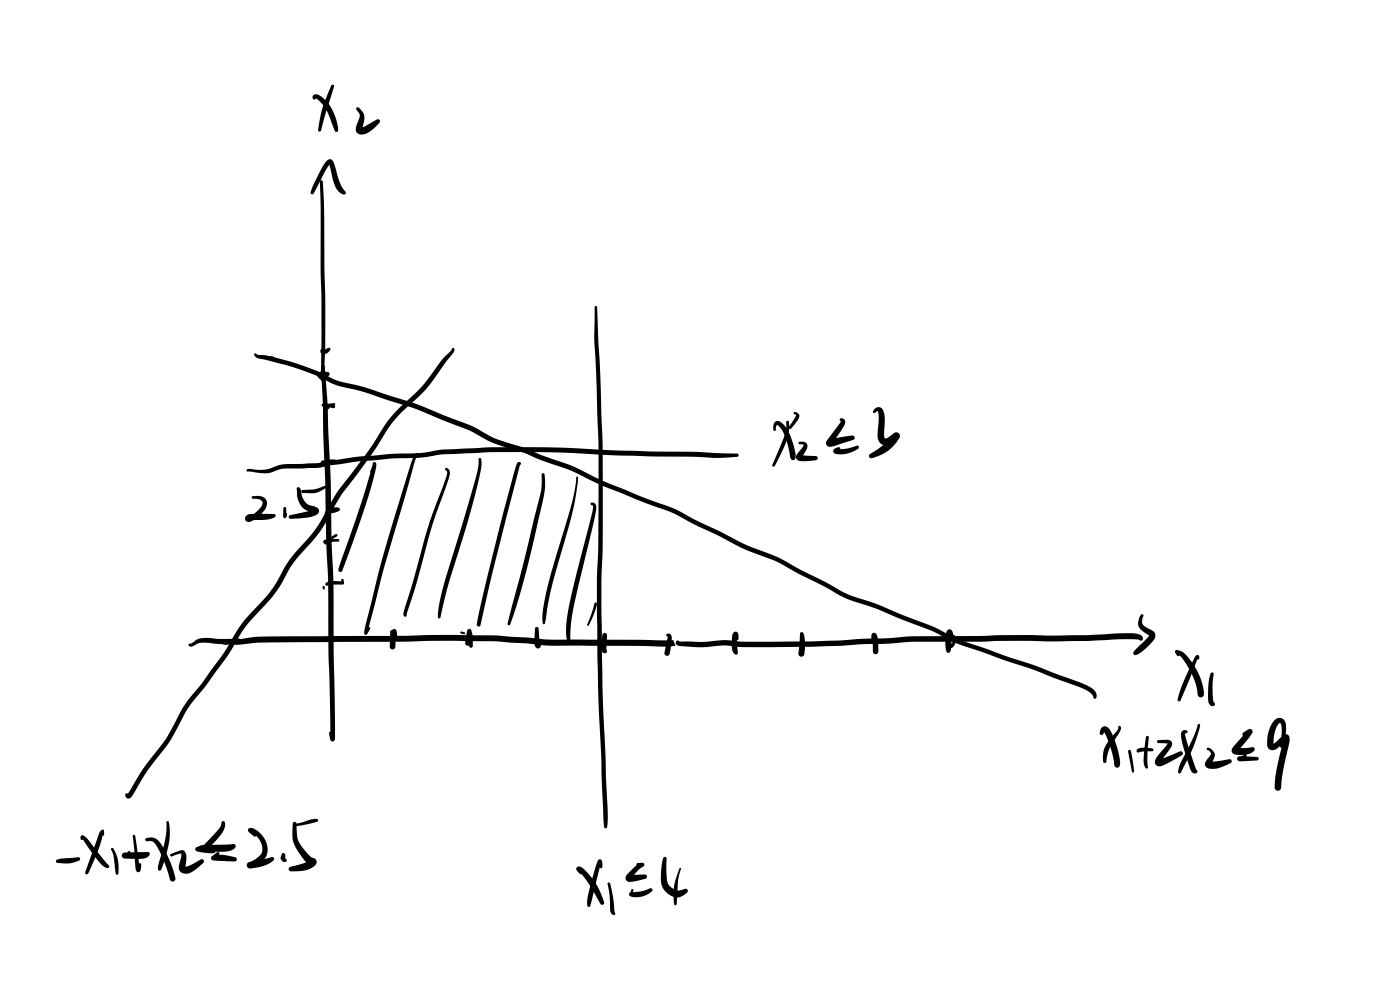
\includegraphics[width=0.7\textwidth]{./pic/pic1.jpeg}
        \caption{}
        \end{figure}

    \textbf{(b)} 转化为如下标准型:
    $$\begin{array}{ll}
        \textrm{maximize} & c^Tx\\
        \textrm{subject to} & Ax=b\\
        & x\geq 0
    \end{array}$$
    其中, $x=\begin{pmatrix}
        x_1\\ \vdots \\x_6
    \end{pmatrix}
    ,c=\begin{pmatrix}
        3\\5\\0\\0\\0\\0
    \end{pmatrix},A=\begin{pmatrix}
        -1 & 1 & 1 & 0 & 0 & 0\\
        1 & 2 & 0 & 1 & 0 & 0\\
        1 & 0 & 0 & 0 & 1 & 0\\
        0 & 1 & 0 & 0 & 0 & 1
    \end{pmatrix},b=\begin{pmatrix}
        2.5\\
        9\\
        4\\
        3
    \end{pmatrix}$

    \textbf{(c)} 由 \textbf{(a)} 中的图可以看出extreme point有\\ $(x_1,x_2)=(0,0),(4,0),(4,2.5),(3,3),(0.5,3),(0,2.5)$ 

    \textbf{(d)} 最优解为 $(x_1,x_2)=(4,2.5)$ ,取到的最优值为 $24.5$
\end{problem}

\begin{problem}

    \textbf{(a)} 由于 $e^Tx=1\Leftrightarrow \sum_ix_i=1$ ,因此 $c^Tx=\sum_ic_ix_i\geq \sum_i (\min_ic_i)x_i=\min_ic_i\sum_ix_i=\min_ic_i$ 。令 $k=\arg\min_ic_i$ (有多个则任取一),则 $x_k=1,x_i=0,\forall i\neq k$ 时可以取到极值。\\
    若限制改为 $e^Tx\leq 1$ ,则有 $c^Tx\geq \sum_i(\min_ic_i)x_i=\min_ic_i\sum_ix_i$ 。又由于有 $0\leq \sum_ix_i\leq 1$ ,故当 $\min_ic_i\geq 0$ 时,有 $c^Tx\geq \min_ic_i\sum_ix_i\geq 0$ ,当 $x_i=0,\forall i$ 时取到等号。当 $\min_ic_i< 0$时,则有 $c^Tx\geq \min_ic_i\sum_ix_i\geq \min_ic_i$ ,令 $k=\arg\min_ic_i$ (有多个则任取一),当 $x_k=1,x_i=0,\forall i\neq k$ 时可以取到极值。

    \textbf{(b)} 当 $\beta$ 是 $0$ 到 $n$ 之间的整数时,不妨令 $c^T=(c_1,\cdots,c_n)$ 且 $c_{(1)},\cdots ,c_{(n)}$ 为 $c_i$ 从小到大排序后的值。那么有 $c^Tx\leq \sum_{i=1}^\beta c_{(i)}$。当排序后 $c_i$ 的下标小于等于 $\beta$ 时 $x_i=1$ ,否则 $x_i=0$\\
    若限制改为 $\beta$ 不是整数。则有 $c^Tx\leq \sum_{i=1}^{[\beta]}c_{(i)}+\{\beta\}c_{[\beta]+1}$ 。当排序后 $c_i$ 的下标小于等于 $[\beta]$ 时 $x_i=1$ ,当 $c_i$ 排序后下标为 $[\beta]+1$ 时 $x_i=\{\beta\}$ ,否则 $x_i=0$\\
    若限制改为 $e^Tx\leq \beta$ ,那么有 $c^Tx\leq \sum_{i=1}^\beta \min(c_{(i)},0)$。当 $c_i<0$ 且排序后 $c_i$ 的下标小于等于 $\beta$ 时 $x_i=1$ ,否则 $x_i=0$\\
\end{problem}

\begin{problem}

    由 $Ax\leq b$ 可转化成 $Ax+s=b$ ,则原来的条件 $Ax\leq b,Cx=d$ 可转化为如下形式:
    $$\begin{pmatrix}
        A & I_4\\C & 0
    \end{pmatrix}\begin{pmatrix}
        x\\s
    \end{pmatrix}=\begin{pmatrix}
        b\\d
    \end{pmatrix}$$
    其中 $\begin{pmatrix}
        A & I_4\\C & 0
    \end{pmatrix}$ 为 $5\times 8$ 的矩阵,秩为 $5$ 。选取 $s_2=s_3=s_4=0$ ,可解得 $x_1=x_2=x_3=x_4=s_1=1$ 为一个feasible solution。故 $x^*=(1;1;1;1)$ 为一个extreme point。
\end{problem}

\begin{problem}

    线性规划为标准型,其中有 $A=\begin{pmatrix}
        1 & 0 & 4 & 0 & \alpha\\
        0 & 1 & -1 & 0 & \beta\\
        0 & 0 & 2 & 1 & \gamma
    \end{pmatrix}$,不难发现该矩阵行满秩。故存在最优的基解。
\end{problem}

\begin{problem}
    
    \textbf{(a)} 其中(1)等价于 $Ax>0$ ,可以转化成 $-Ax+\alpha e\leq 0,\alpha>0$ ,由Farkas's Lemma,有如下的alternative system: $(A\  e)^Ty=(0\ 1)^T,y\geq 0$ ,等价于 $A^Ty=0,y>0$ 。故得证。

    \textbf{(b)} 考虑如下两个线性规划:
    $$\begin{array}{ll}
        \textrm{minimize} & c^Tx\\
        \textrm{subject to} & Ax=b\\
        & x\geq 0
    \end{array}$$ 以及:
    $$\begin{array}{ll}
        \textrm{maximize} & b^Ty\\
        \textrm{subject to} & A^Ty\leq x
    \end{array}$$
    这两个线性规划互为对偶,并且如果两者都有最优解 $x^*,y^*$ ,则存在 $c^Tx^*=b^Ty^*$ ,符合条件 $c^Tx-b^Ty\leq 0$ 。故该条件即等价于上面两个线性规划都有最优解。对于这两个线性规划的alternative system: $A^Tw\leq 0,b^Tw>0,A^Tz=0,z\geq 0,c^Tw<0$ ,如果题设条件成立,则两个规划均有解,则此条件不成立;如果此条件成立,则两个规划均无解,题设条件不成立,故为alternative system。
\end{problem}

\begin{problem}

    使用cvx求得三个函数为 $f_{ls}(x)=0.5755x+4.1841,f_{l_1}=0.9716x+4.9459, f_{l_\infty}=-0.5249x+3.9335$ 
    对应的三个图像依次如下:
    可以发现对于整体的趋势来说,$l_1$-norm拟合得最好; $l_2$-norm倾向于体现整体的趋势,但由于离群值带来的偏差是平方级别的,所以也会显示出部分离群值带来的影响;而 $l_\infty$-norm由于是取 $\max$ ,显著得受到离群值的影响。
    \begin{figure}[h]
        \centering
        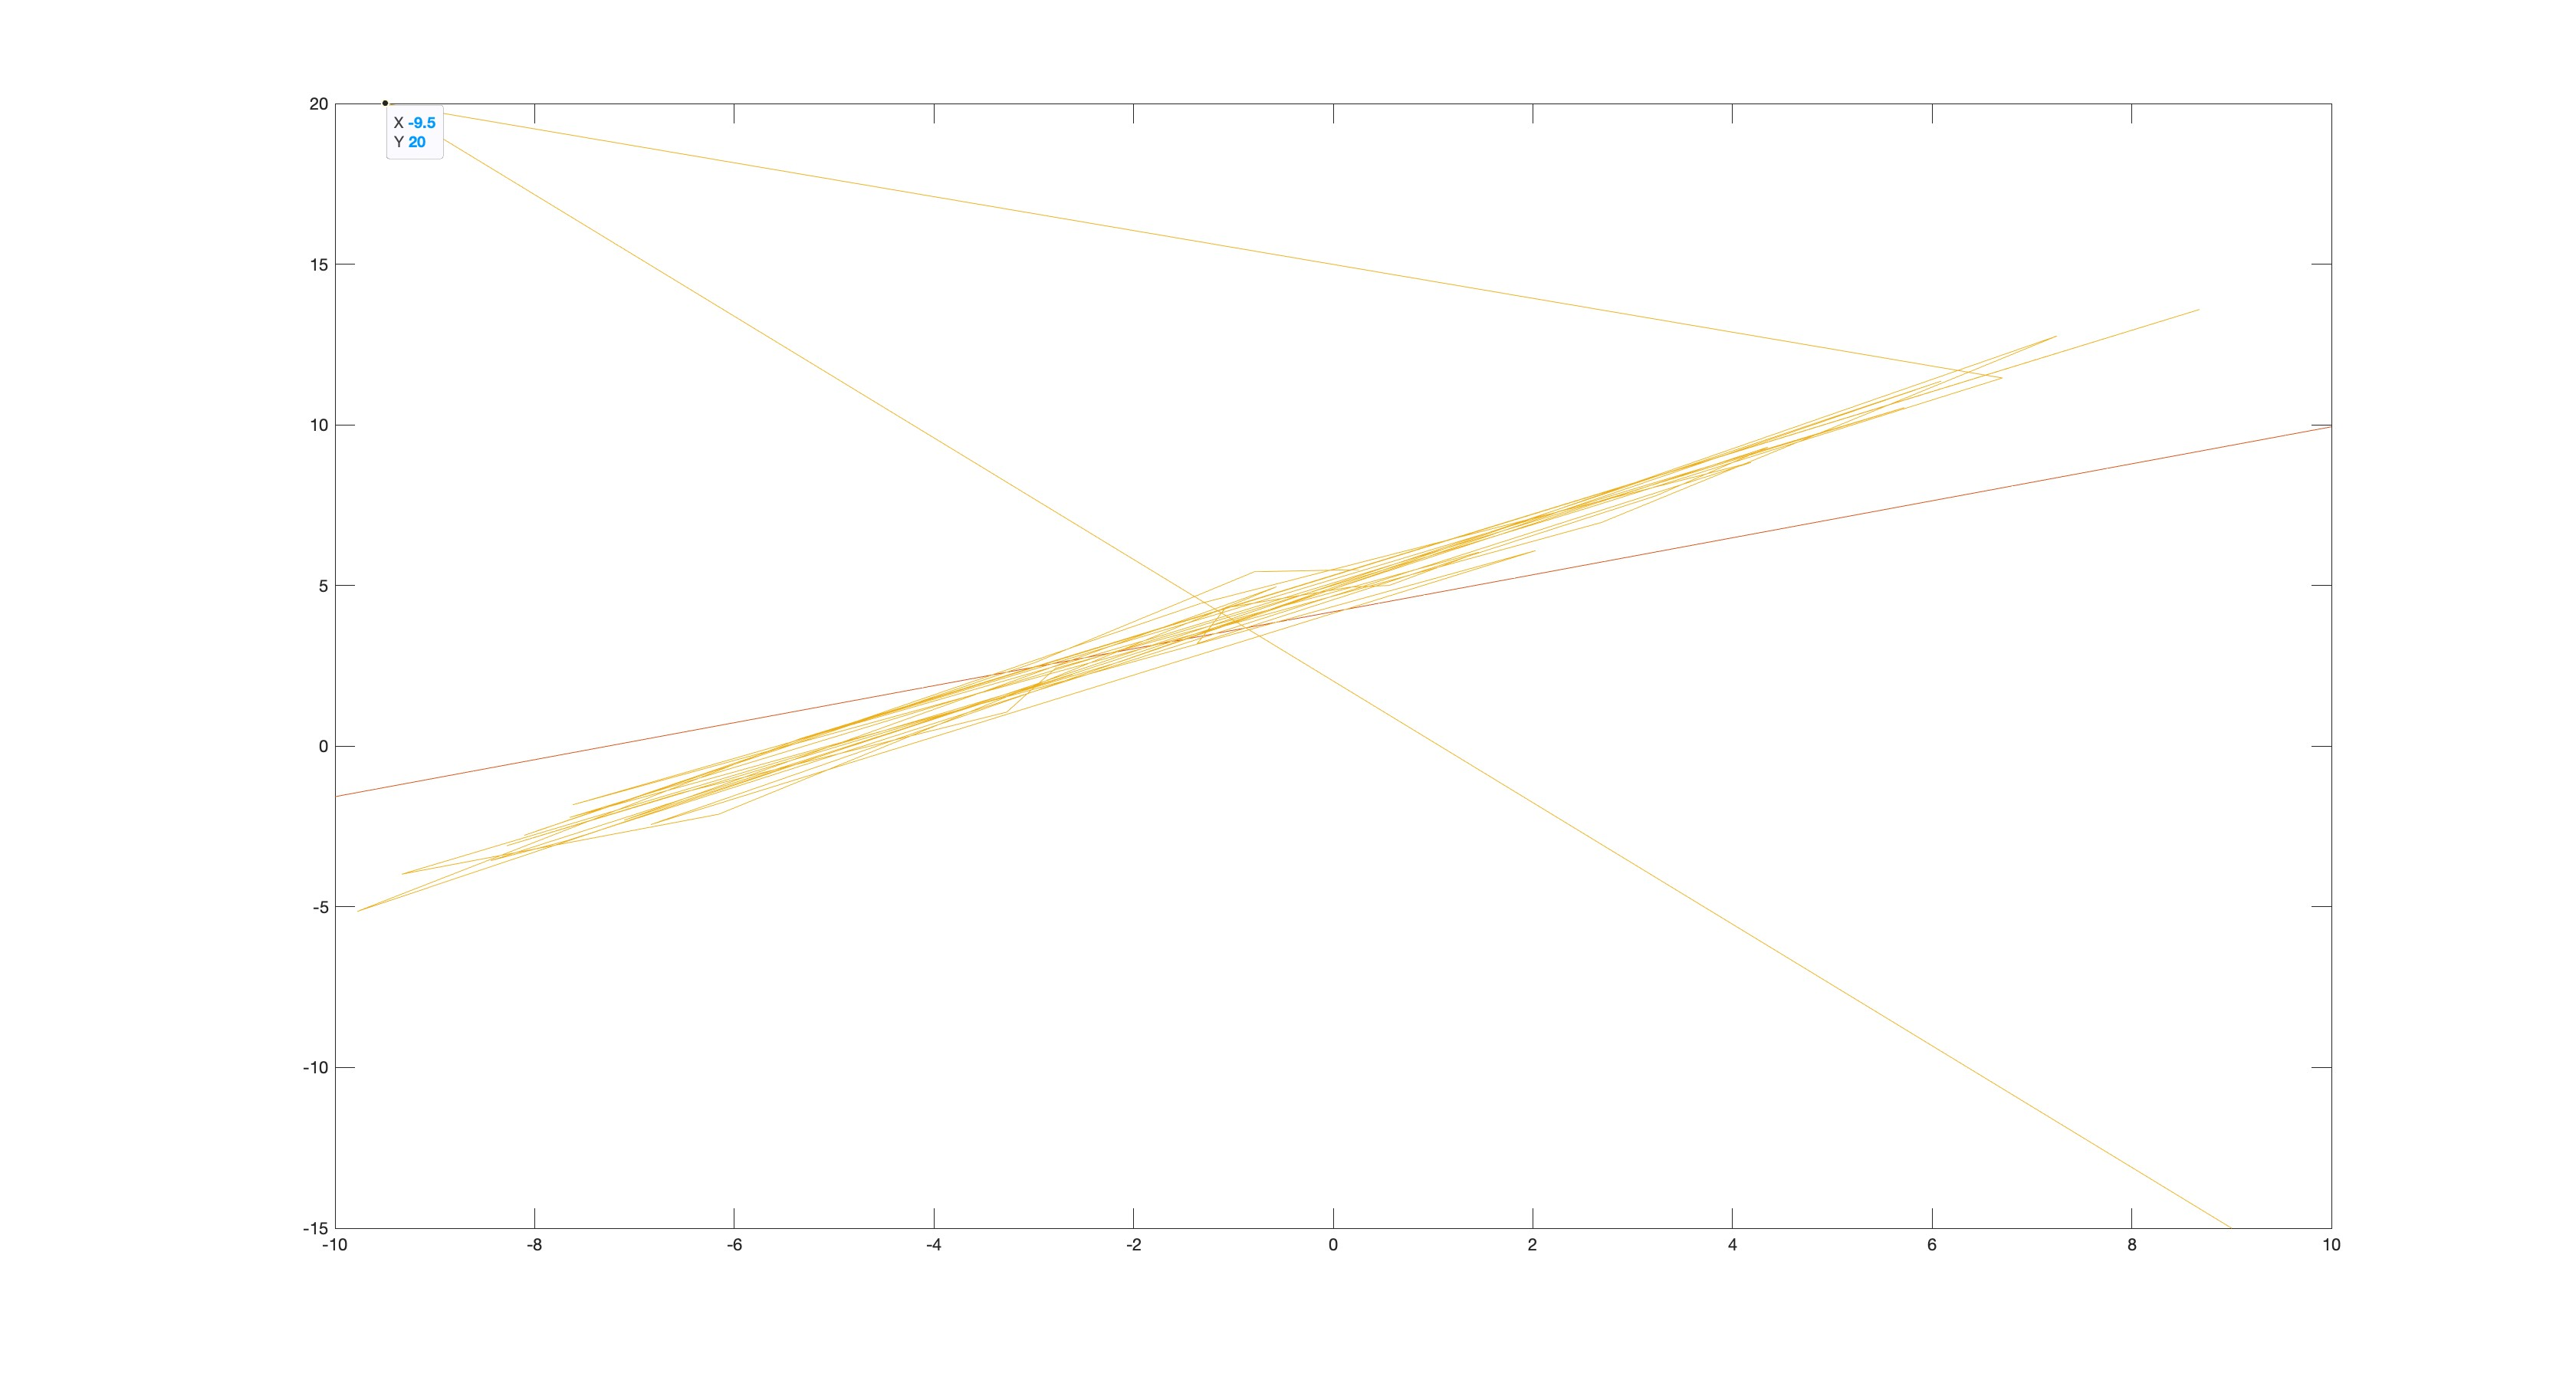
\includegraphics[width=0.95\textwidth]{./pic/pic2.jpg}
        \caption{$f_{ls}(x)$}
    \end{figure}
    \begin{figure}[h]
        \centering
        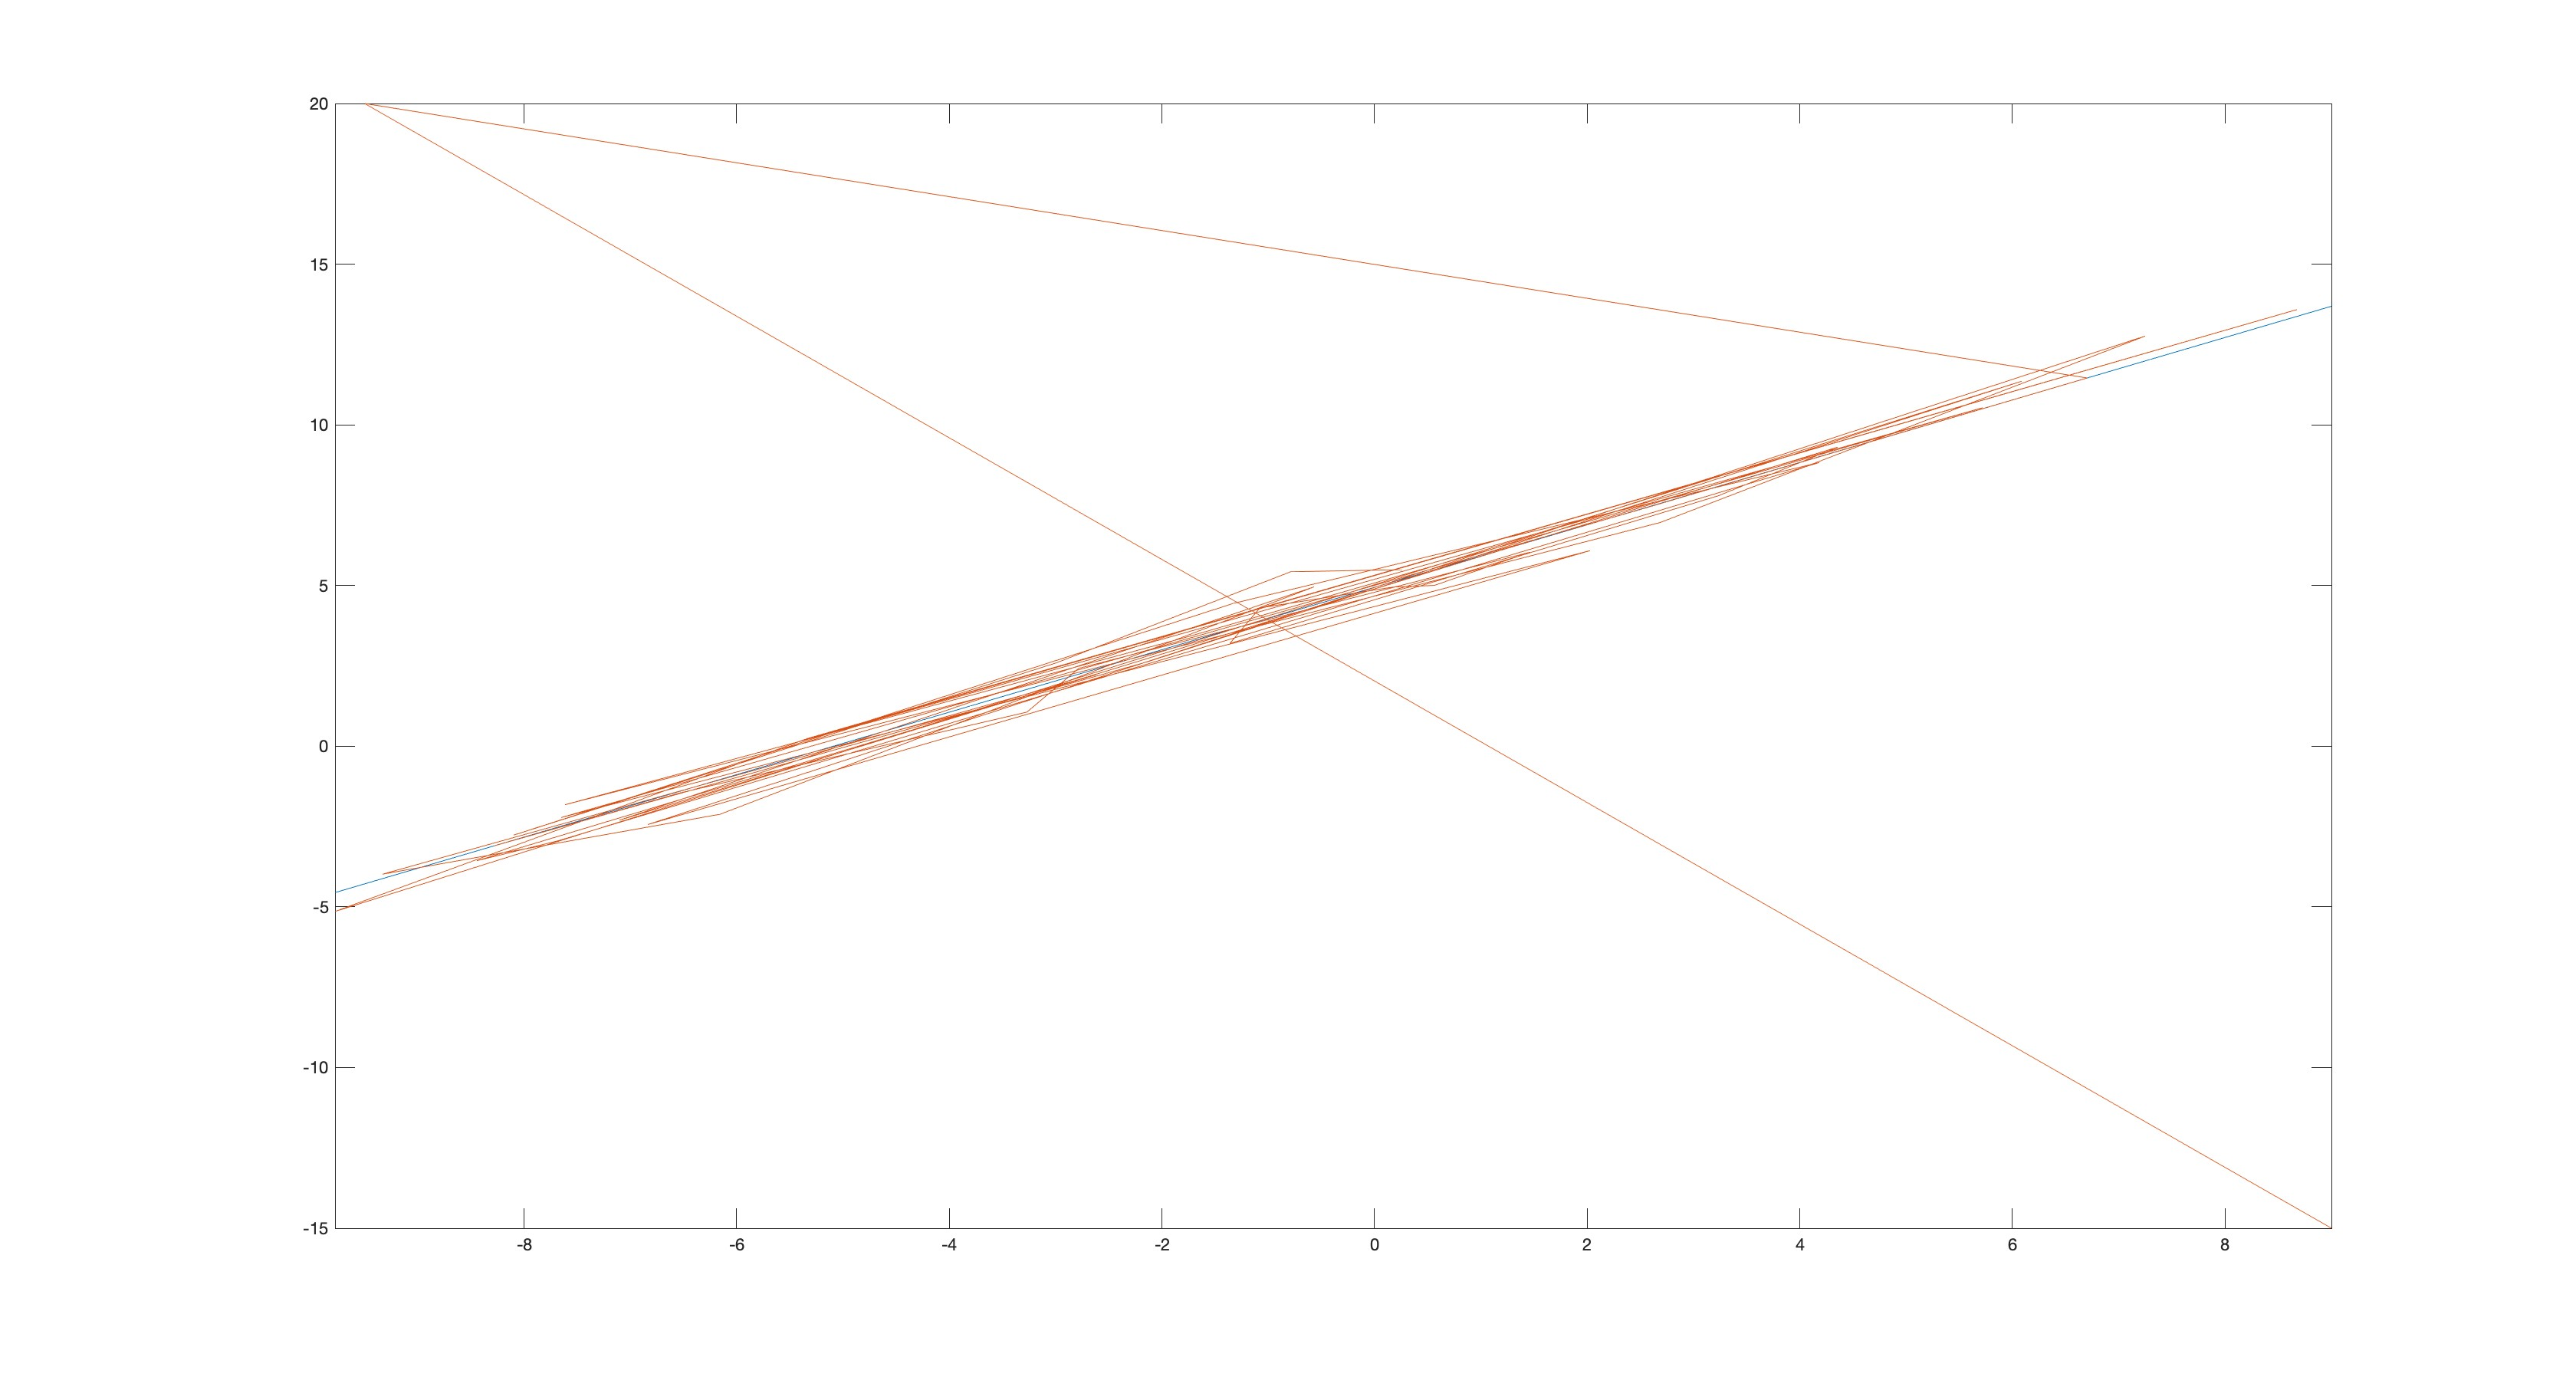
\includegraphics[width=0.95\textwidth]{./pic/pic3.jpg}
        \caption{$f_{l_1}$}
    \end{figure}
    \begin{figure}[h]
        \centering
        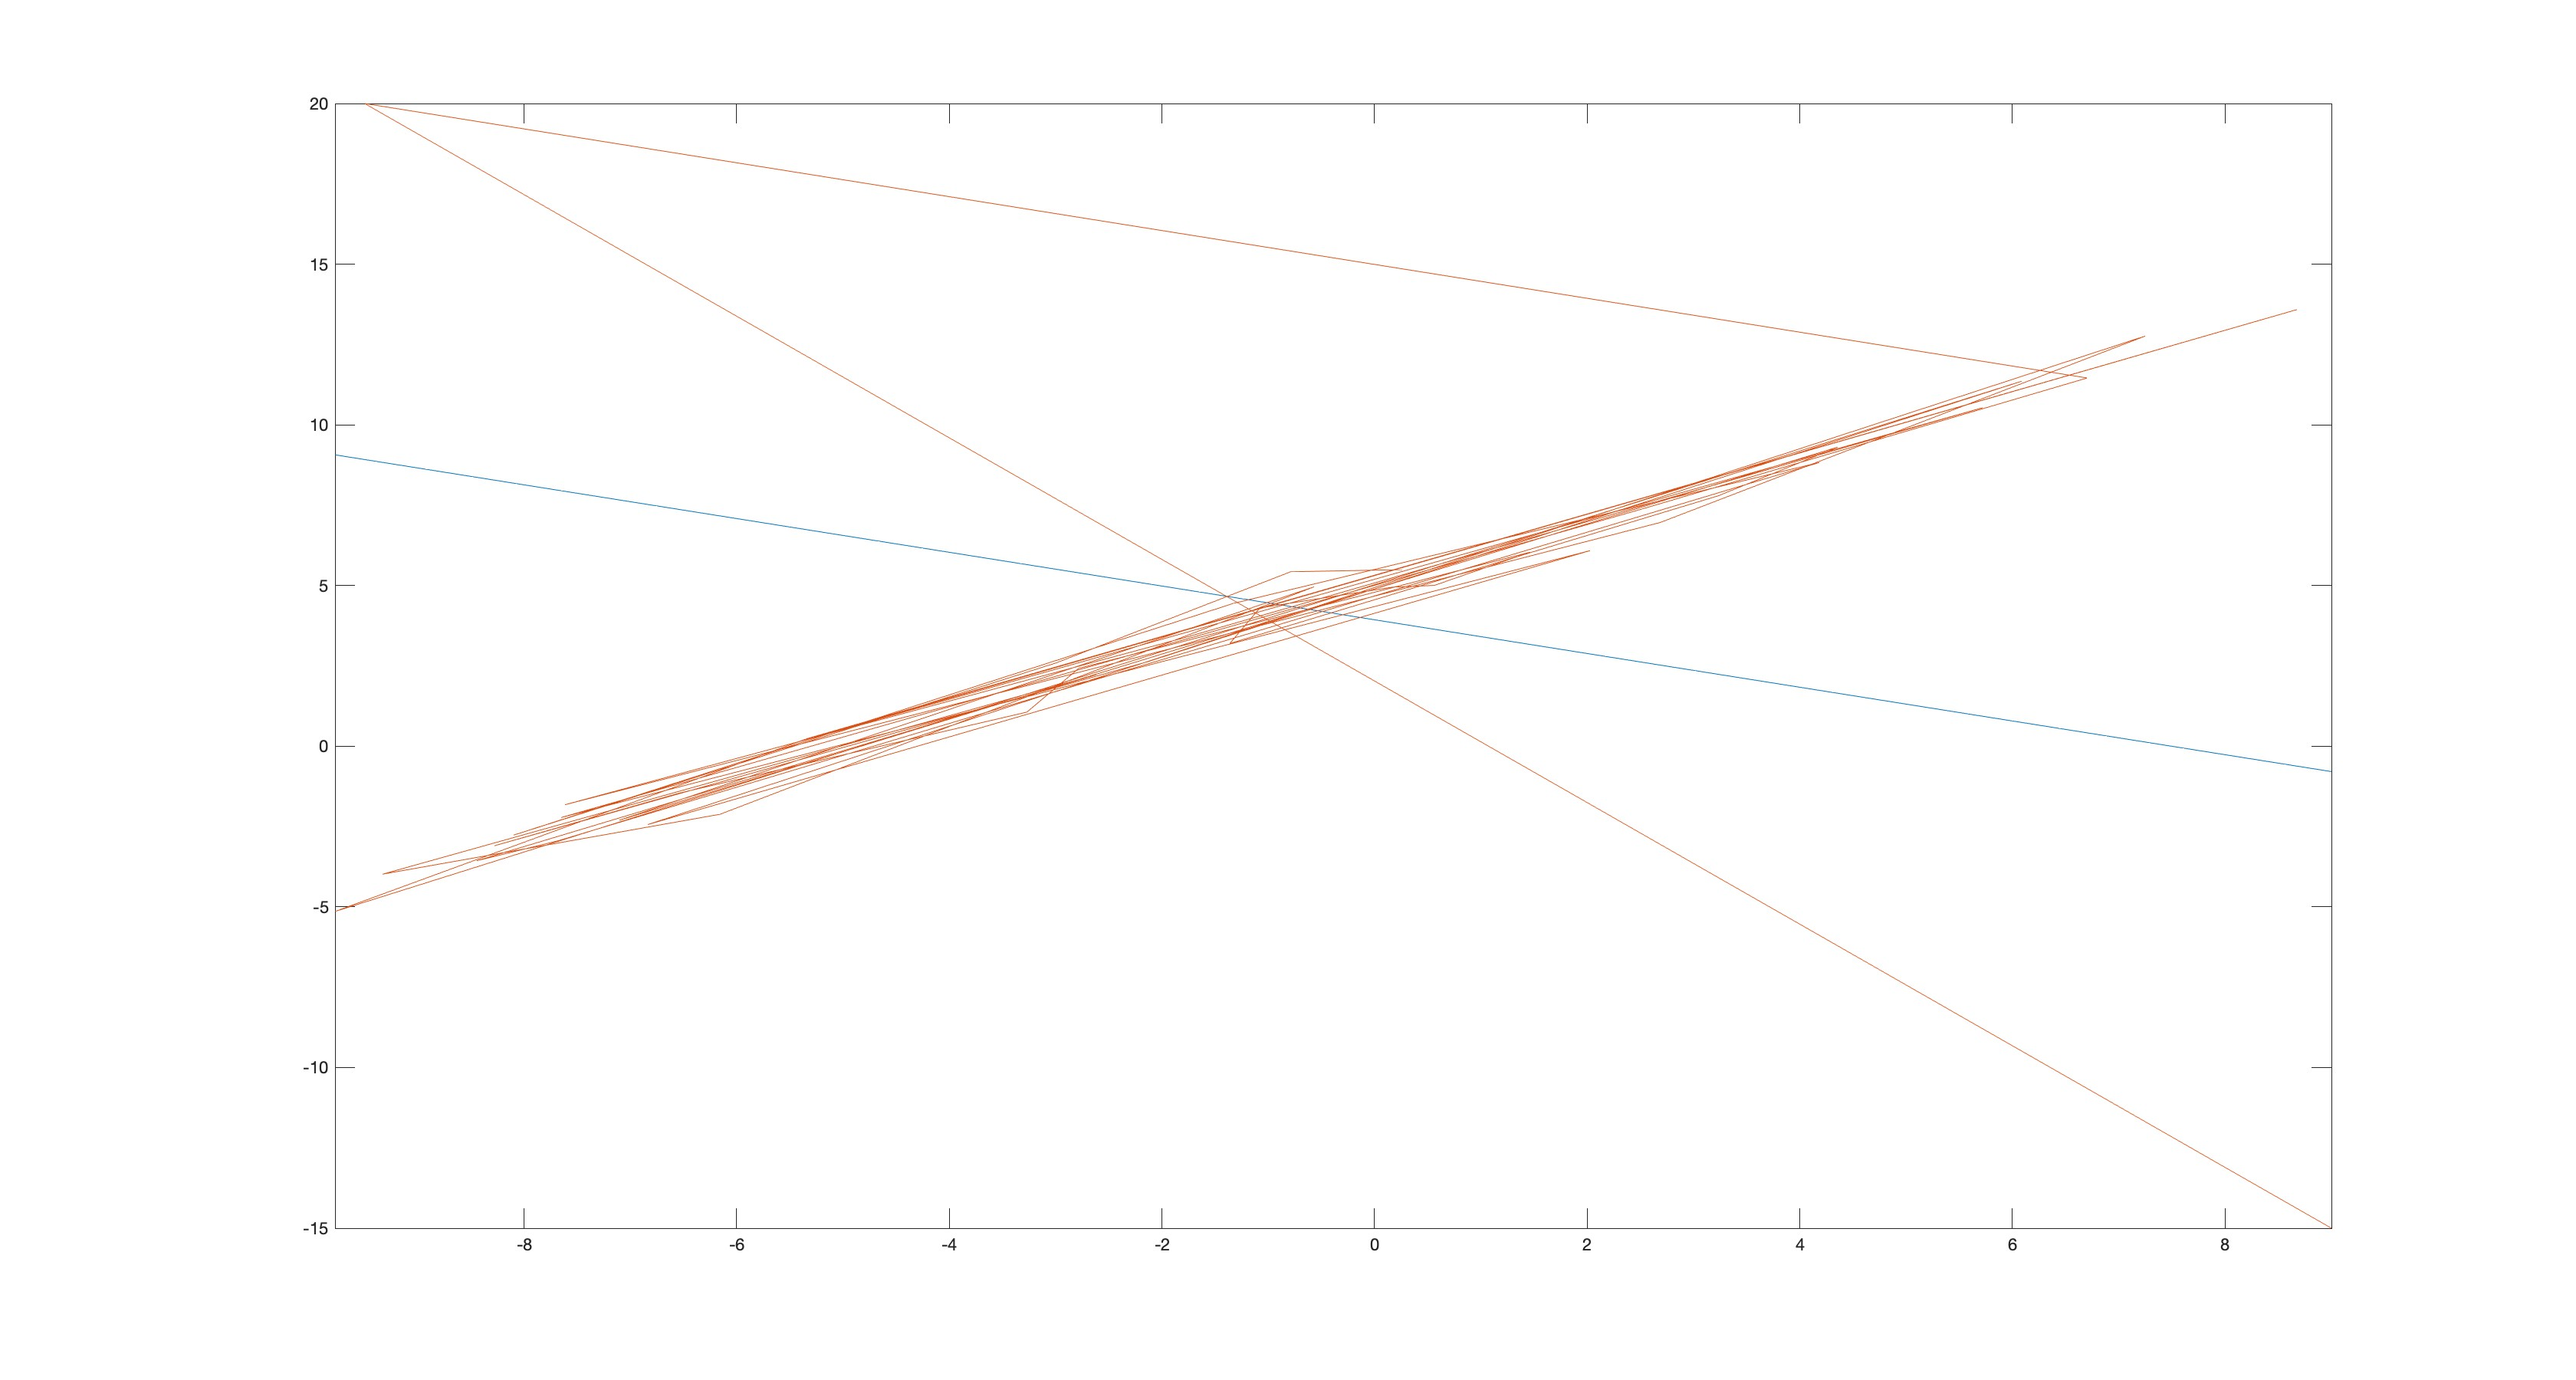
\includegraphics[width=0.95\textwidth]{./pic/pic4.jpg}
        \caption{$f_{l_\infty}$}
    \end{figure}
\end{problem}

\end{document}